\subsubsection*{AML}

\paragraph{Overview}

AML is a memory management library designed to ease the use of complex
memory topologies and complex data layout optimizations for
high-performance computing applications.

AML is a framework providing locality-preserving abstractions to
application developers.  In particular, AML aims to expose flexible
interfaces to describe and reason about how applications deal with data
layout, tiling of data, placement of data across hardware topologies, and
affinity between work and data.

\paragraph{Key Challenges}

Between non-uniform memory access (NUMA) to regular DRAM, the 3-D stacked
high-bandwidth memory, and the memory local to the accelerator devices such
as GPUs, the increasing depth of the memory hierarchy presents exascale
applications with a critical challenge of how to use the available
heterogeneous memory resources effectively.

Standardized interfaces to manage complex memory hierarchies are lacking,
and vendors are reluctant to innovate in this space in the absence of clear
directions from the community.  Coming up with an interface that is
sufficiently expressive to cover the emerging and projected hardware
advances, yet is simple enough and practical to be both acceptable and
useful to the applications is the key challenge that we are working on
addressing.

\paragraph{Solution Strategy}

AML provides explicit, application-aware memory management for deep memory
systems.  It offers a collection of building blocks that
are \emph{generic}, \emph{customizable}, and \emph{composable}.
Applications can specialize the implementation of each offered abstraction
and can mix and match the components as needed.  AML can be used to create,
for example, a software-managed scratchpad for multilevel DRAM hierarchy
such as HBM and DDR.  Such a scratchpad provides applications with a memory
region with a predictable high performance for critical data structures.

We provide applications and runtimes with a descriptive API for data
access, where all data placement decisions are explicit, and so is the
movement of data between different memory types.  At the same time, the API
does abstract the memory topology and other device complexities.  We focus
on optimizing data locality for current and future hardware generations;
applications provide insights for static allocations, and we can also
dynamically and asynchronously move or transform data to optimize for a particular 
device or to best take advantage of the memory hierarchy.

\begin{wrapfigure}[6]{r}{.18\textwidth}
%\vspace{-12pt}%
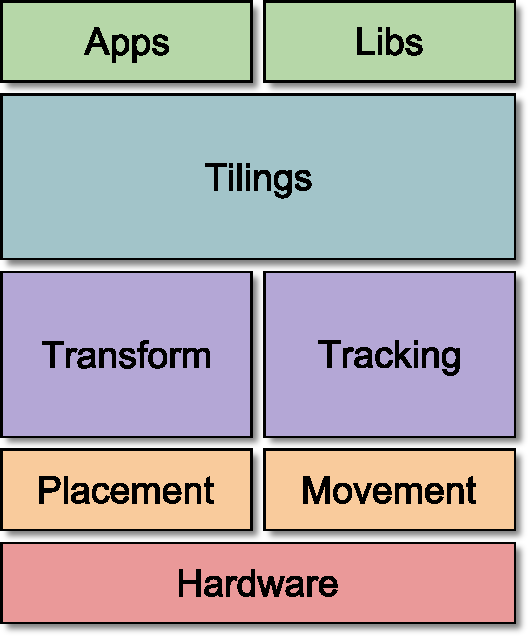
\includegraphics[width=.18\textwidth]{projects/2.3.1-PMR/2.3.1.19-Argo-PowerSteering/aml-components}
\end{wrapfigure}
The figure on the right depicts the major components of AML, including:
\begin{itemize}
\item Topology and hardware management (dependent on NUMA, hwloc, and SICM)
\item Data layout descriptions (application-specific)
\item Tiling schemes (including ghost areas)
\item Data movement facilities (currently primarily \texttt{memcpy})
\item Pipelining helpers (scratchpad, asynchronous requests)
\end{itemize}

\paragraph{Recent Progress}

%We developed AML, a memory library for explicit management of deep memory
%architectures.  Its main feature is a flexible and composable API, allowing
%applications to implement algorithms similar to out-of-core for deep
%memory.  We provided multiple optimized versions of memory migration
%facilities, ranging from a regular copy to a transparent move of memory
%pages, using synchronous and asynchronous interfaces and single- and
%multithreaded backends.  We validated the initial implementation on Intel's
%Knights Landing using a pipelining scheme for stencil applications.  We
%also identified interaction points between UMap and AML.  Further
%performance and capability improvements are underway.  In particular, we
%performed exhaustive studies comparing performance of various approaches
%for block-based DGEMM and task-based Cholesky decomposition.

AML development reached its first stable release recently.  We have a custom CI
pipeline in place that ensures this stability via automated testing (we are
making progress on leveraging the ECP CI infrastructure as well).  The
source code of version 0.1.0 is available on our website; we also provide
documentation on ReadTheDocs.  AML can also be installed via Spack.

We have been collaborating with the ExaSMR project on improving the
performance of the XSBench and RSBench proxy apps.  We applied the
topology-aware data replication facilities of AML in order to replicate
read-only and latency-sensitive data on low-latency memory nodes, improving
the code's behavior on NUMA architectures.  We found the effort to have a
limited impact on the application code, provided that the data is correctly
structured.  Performance was tested on four x86 architectures: Intel's
Knights Landing, Skylake, and Haswell, as well as AMD's Epyc.
Figure \ref{fig:argo:aml-results} outlines the results of these
experiments.

\begin{figure}
\centering
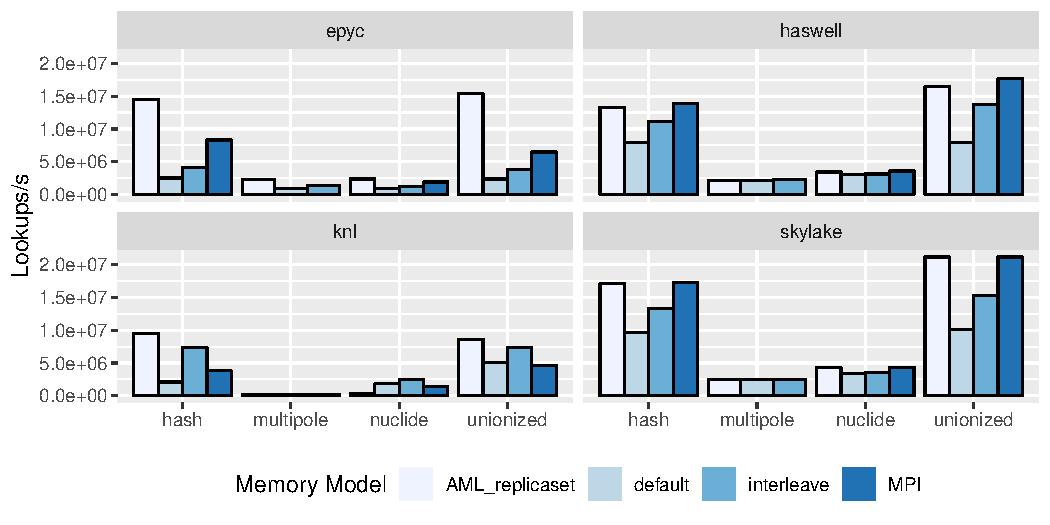
\includegraphics[width=.8\textwidth]{projects/2.3.1-PMR/2.3.1.19-Argo-PowerSteering/aml-results}
\caption{Impact of the memory management policy used on the performance of
proxy apps.}
\label{fig:argo:aml-results}
\end{figure}


\paragraph{Next Steps}

We want to add support for more types of memory through the integration
with UMap and with other projects such as SICM.  We are planning to
significantly increase the topology-awareness of our interface through the
integration with Hwloc, by providing support for GPUs and other
accelerators and their topologies, and by extending the interface with
performance-oriented topology queries.  We are engaged in Aurora co-design
effort to ensure suitable hardware support on that platform.  Our
positive early results with ExaSMR proxy apps will be expanded to cover
the actual OpenMC application.
